\documentclass[11pt]{article}

\usepackage[margin=1in]{geometry}
\usepackage{graphicx}
\usepackage{booktabs}
\usepackage{amsmath}
\usepackage{caption}
\usepackage[hidelinks]{hyperref}
\usepackage{times}

\setlength{\parindent}{0pt}
\setlength{\parskip}{0.72em}
\captionsetup{font=small,labelfont=bf,skip=4pt}
\renewcommand{\arraystretch}{1.08}

% Let figures share pages with text rather than floating onto pages of their own.
\renewcommand{\topfraction}{0.92}
\renewcommand{\bottomfraction}{0.85}
\renewcommand{\textfraction}{0.06}
\renewcommand{\floatpagefraction}{0.80}

\title{\vspace{-2em}Spending a Fixed Compute Budget:\\
Agents, Rounds, Reasoning Depth, and Sampling}
\author{Study \texttt{openrouter\_agent\_allocation\_v1}}
\date{17 September 2026}

\begin{document}
\maketitle
\vspace{-1.5em}

\section*{Abstract}
\addcontentsline{toc}{section}{Abstract}

A fixed inference budget can be spent in several ways. It can buy more agents working in
parallel, more rounds of revision, a longer reasoning allowance inside a single call, or simply
more independent samples read out by a vote. This report asks which of those purchases is worth
making, holding total compute exactly constant.

We define the budget as $C = B \cdot R \cdot A$, the product of the number of agents, the number
of rounds, and the per-agent per-round reasoning allowance. The study evaluated 95 configurations
on one fixed 400-item panel spanning four benchmarks, with 67{,}514 graded generations and a
25-sample independent bank per item that makes oracle pass@$k$ available at every budget. Because
$C$ is materialised per configuration, allocations that differ in shape but agree in cost can be
compared directly. At $C = 8A$, for instance, seven distinct allocations were run.

Three findings hold across benchmarks. First, at matched compute the shape of the allocation
barely matters: of 70 per-benchmark comparisons against independent sampling at the same budget,
none survives multiplicity correction, and the largest effect anywhere is 6 accuracy points.
Second, every allocation plateaus near what two samples and a vote already deliver, while oracle
pass@$k$ continues to climb, so the headroom that compute makes available but no configuration
collects grows from zero to 6.7 accuracy points on the three-benchmark macro and to 9 points on
MMLU-Pro. Third, letting agents see each other's work actively destroys accuracy, and the damage
grows with rounds: at five agents and four peer rounds the penalty is 5.0 points on the macro and
10 points on MBPP+.

The binding constraint in this regime is not generation but selection. Going from one sample to
twenty-five moves 16 points of MMLU-Pro items out of the state where no correct answer exists, but
only 1.1 of those points end up in a state a vote can deliver; the other 15 land in a state where
the correct answer is present and outvoted.

We then ask which axis would collapse that gap. Ranking the levers on the same sealed data, a
reranker with pairwise AUC 0.70 applied to candidates the run already paid for beats every one of
the 95 allocations, and AUC 0.80 delivers 0.876 against an oracle of 0.917; today's plurality vote
is equivalent to AUC 0.63. A larger per-draw reasoning allowance is the only generation-side lever
that helps, halving the MATH-500 gap. More agents and more rounds contribute close to nothing.
The prescription is to spend on verification, not on allocation.

\section{Methods}

\subsection{Model, benchmarks and panels}

Generations come from \texttt{google/gemini-2.5-flash-lite} through OpenRouter with the provider
pinned, fallbacks disabled and caching off, at temperature 0.7 with nucleus sampling at 0.95. A replication arm
uses \texttt{google/gemini-2.5-flash}.

Four benchmark families are scored: MATH-500 with \texttt{math\_verify}, MMLU-Pro with exact
option match, a four-subtask zero-shot BBH subset (logical deduction, shuffled objects, boolean
expressions, temporal sequences) with exact task match, and MBPP+ graded by the full EvalPlus
suite. BBH is reported as this four-subtask subset, not the official full BBH score, and its
aggregate weights the four subtasks equally.

The main panel is 400 items, 100 per benchmark. A high-allowance panel of 96 items and a
replication panel of 48 items are nested subsets of it, so every cross-panel comparison uses
shared item ids only. All 95 main-panel configurations share one fixed item population, which is
what allows every contrast in this report to be paired item by item.

\subsection{The compute accounting}

Each configuration is a triple $(B, R, A)$ and the budget is their product. The sealed tables
carry $B$, $R$ and $A$ as explicit columns, so no parsing of configuration names is involved:

\begin{center}
\small
\begin{tabular}{llccl}
\toprule
Family & Notation & $B$ & $R$ & $C$ \\
\midrule
Independent samples, vote & \texttt{sample/k} & $k$ & 1 & $k A_0$ \\
One agent revising & \texttt{private\_single/t} & 1 & $t$ & $t A_0$ \\
Team, no peer exposure & \texttt{private\_team/n/r} & $n$ & $1+r$ & $n(1+r) A_0$ \\
Team, peer exposure & \texttt{peer/n/r} & $n$ & $1+r$ & $n(1+r) A_0$ \\
One deeper call & \texttt{deep/m} & 1 & 1 & $m A_0$ \\
\bottomrule
\end{tabular}
\end{center}

$A_0$ is 1024 tokens on the main panel and 4096 on the high panel. The \texttt{deep} family scales
$A$ rather than the call count, so its budget must be read from $A$ and not from the number of
generations; a build-time check asserts that the derived $C$ equals the sealed requested reasoning
tokens for every configuration on every panel, and that $B \cdot R$ equals the sealed generation
count everywhere except \texttt{deep}, where it is one call by construction.

Figure~\ref{fig:design} shows the resulting design. Fourteen budget levels carry two or more
distinct allocations, and the levels $C/A_0 \in \{4, 8\}$ carry seven each.

\begin{figure}[htbp]
\centering
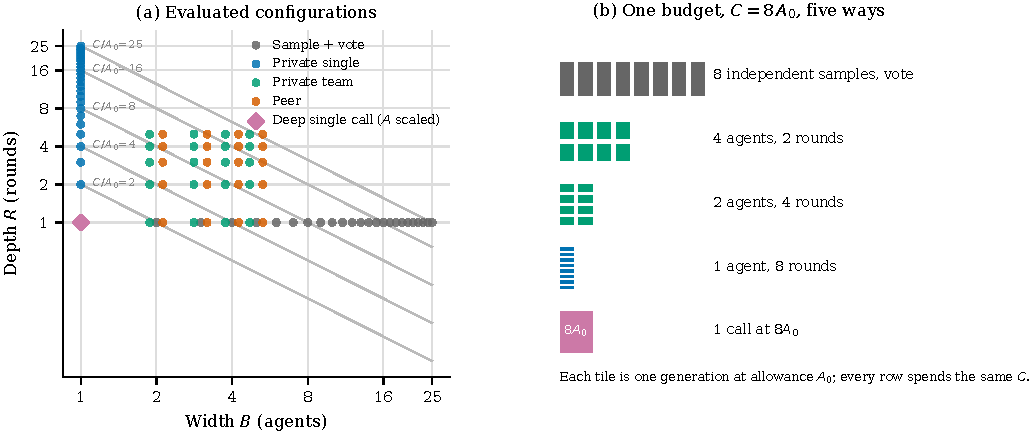
\includegraphics[width=\textwidth]{figures/f1_design_map.pdf}
\caption{The design. (a) Every evaluated configuration in the width-depth plane; grey lines are
iso-compute contours, along which every point spends the same $C$. Private-team and peer points
are nudged apart because they occupy identical $(B, R)$ cells and differ only in whether agents
see each other. (b) The five ways one budget of $8A_0$ was actually spent.}
\label{fig:design}
\end{figure}

\subsection{What counts as a result, and what does not}

A configuration delivers exactly one answer per item. Text benchmarks select it by plurality vote;
MBPP+ selects by prompt-visible public tests only, and is therefore reported as
\texttt{public\_select@k} and never as a vote. Delivered accuracy counts operational failures,
unparseable outputs and abstentions as incorrect, so nothing is silently dropped.

Oracle pass@$k$ is not an available selector. It is reported as a ceiling only, using the standard
combinatorial estimator $1 - \binom{n-c}{k} / \binom{n}{k}$ over the 25-sample bank. Two normalised
quantities are used throughout:

\textbf{Amplification} is delivered accuracy minus the accuracy of independent sampling at the same
budget, in accuracy points, paired per item. It answers whether an allocation beats simply drawing
$k = C/A_0$ samples and reading them out.

\textbf{Ceiling capture} is $\eta = (\text{accuracy} - \text{pass@1}) / (\text{coverage@}k -
\text{pass@1})$, the share of the headroom that the budget makes available which the configuration
actually delivers. The denominator is the realised prefix coverage of the same $k$ samples, which
is binary per item and therefore pairs with the numerator under the same resample indices. A value
of 1 means the configuration collected everything the budget put within reach; 0 means it did no
better than one sample. Values above 1 are possible and meaningful, because a revising or
communicating configuration can produce an answer that independent sampling never generated. We
suppress $\eta$ where the denominator falls below 0.02, which masks BBH entirely.

\subsection{Estimation and multiplicity}

All intervals are percentile intervals from a 10{,}000-replicate item-clustered bootstrap,
stratified by benchmark and with BBH subtasks weighted equally. Every configuration shares the same
resample indices, so differences between configurations are correctly paired.

Two contrasts were prespecified and frozen before collection: peer versus private team at $B{=}4$,
$r{=}4$, and the communicate-then-private decomposition at $h{=}3$. Those carry Holm-corrected
$p$-values and are quoted directly from the sealed contrast table. Everything else in this report
is exploratory. In the amplification matrix we mark cells whose nominal paired interval excludes
zero, and we also report how many survive Benjamini-Hochberg control within each panel, which
turns out to be the more informative number.

Macro averages are reported two ways: over all four benchmarks, which reconciles with the run
report, and over the three informative ones. BBH is saturated at 1.000 in every configuration, so
including it inflates the level and compresses every contrast toward zero.

\subsection{Limitations}

$A$ is a requested allowance, not realised reasoning; realised token counts are recorded separately
and are consistently below the request. This is a token-accounted and dollar-accounted study, not a
FLOP-matched one. With 100 items per benchmark, one item is one accuracy point, so differences
below roughly 3 points are not separable from noise. Results are from a single small model, and the
peer-communication finding in particular should not be assumed to transfer to larger models. The
text completion headroom was amended twice during piloting, from 1024 to 2048 to 4096 tokens, and
the main run was collected at 4096 under a clarified system prompt. Frontiers shown here are
descriptive: the best among evaluated configurations on this sample, never a validated policy.

\section{Results}

\subsection{Allocation shape barely matters; the ceiling keeps rising}

Figure~\ref{fig:ladder} is the headline. On every benchmark the oracle ceiling climbs steadily with
compute while every delivered curve flattens almost immediately.

\begin{figure}[htbp]
\centering
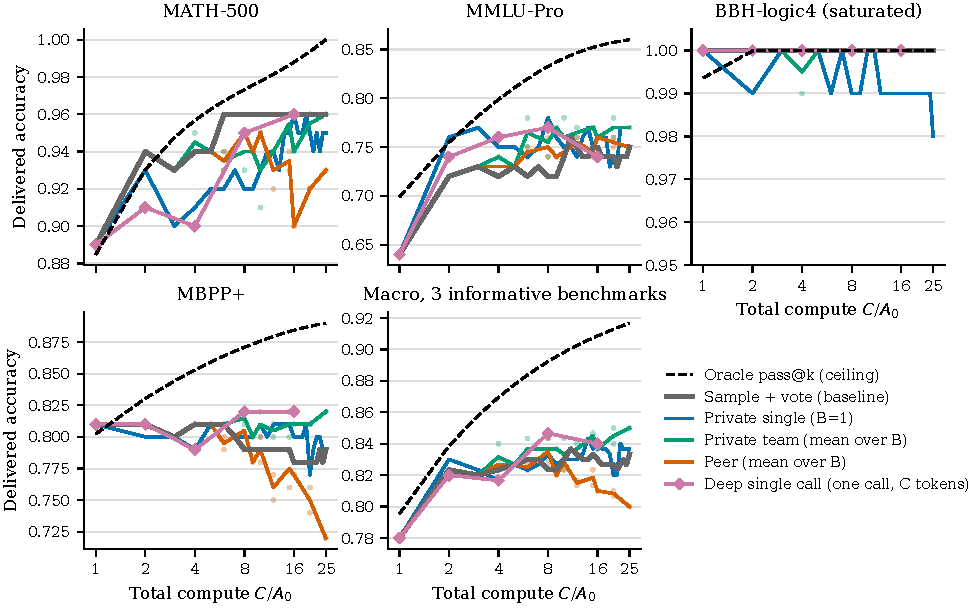
\includegraphics[width=\textwidth]{figures/f2_isocompute_ladder.pdf}
\caption{Delivered accuracy against total compute. All curves at a given $x$ spend the same budget.
The dashed ceiling is oracle pass@$k$, an unavailable selector. Faint points are individual team
sizes; family lines are the mean over $B$. BBH is drawn on a fixed window because it is saturated.}
\label{fig:ladder}
\end{figure}

On the three-benchmark macro a single sample delivers 0.780 and two samples with a vote deliver
0.823. Twenty-five samples deliver 0.833, an additional 1.0 point for twelve times the compute. The
best configuration anywhere in the design is a five-agent private team with three revision rounds
at 0.850, which is 2.7 points above sample-and-vote at a comparable budget and 7.0 points above one
sample. Over the same range oracle pass@$k$ rises from 0.780 to 0.917.

Per benchmark the picture differs in an instructive way. On MATH-500 plain sampling is essentially
unbeatable: it reaches 0.960, which is the best value any configuration attains, while the oracle
reaches 1.000. On MMLU-Pro allocation helps most, with a three-agent private team at one revision
round reaching 0.780 against 0.720 for two samples. On MBPP+ the achievable readout actually
\emph{declines} with budget, from 0.810 at one sample to 0.790 at twenty-five, while oracle coverage
rises to 0.890: selecting code by prompt-visible tests gets worse as the candidate pool grows,
because a candidate that passes the visible assertion and fails the hidden suite becomes easier to
find.

\begin{tabular}{lrrrrrrr}
\toprule
Benchmark & pass@1 & vote@2 & vote@25 & best any & best archive & oracle@25 & headroom \\
\midrule
MATH-500 & 0.890 & 0.940 & 0.960 & 0.960 & 0.960 & 1.000 & 0.040 \\
MMLU-Pro & 0.640 & 0.720 & 0.750 & 0.780 & 0.780 & 0.860 & 0.090 \\
BBH-logic4 & 1.000 & 1.000 & 1.000 & 1.000 & 1.000 & 1.000 & 0.000 \\
MBPP+ & 0.810 & 0.810 & 0.790 & 0.820 & 0.854 & 0.890 & 0.070 \\
Macro (3) & 0.780 & 0.823 & 0.833 & 0.850 & 0.861 & 0.917 & 0.067 \\
\bottomrule
\end{tabular}


\subsection{The amplification matrix}

Figure~\ref{fig:matrix} places every allocation against independent sampling at the same budget.

\begin{figure}[htbp]
\centering
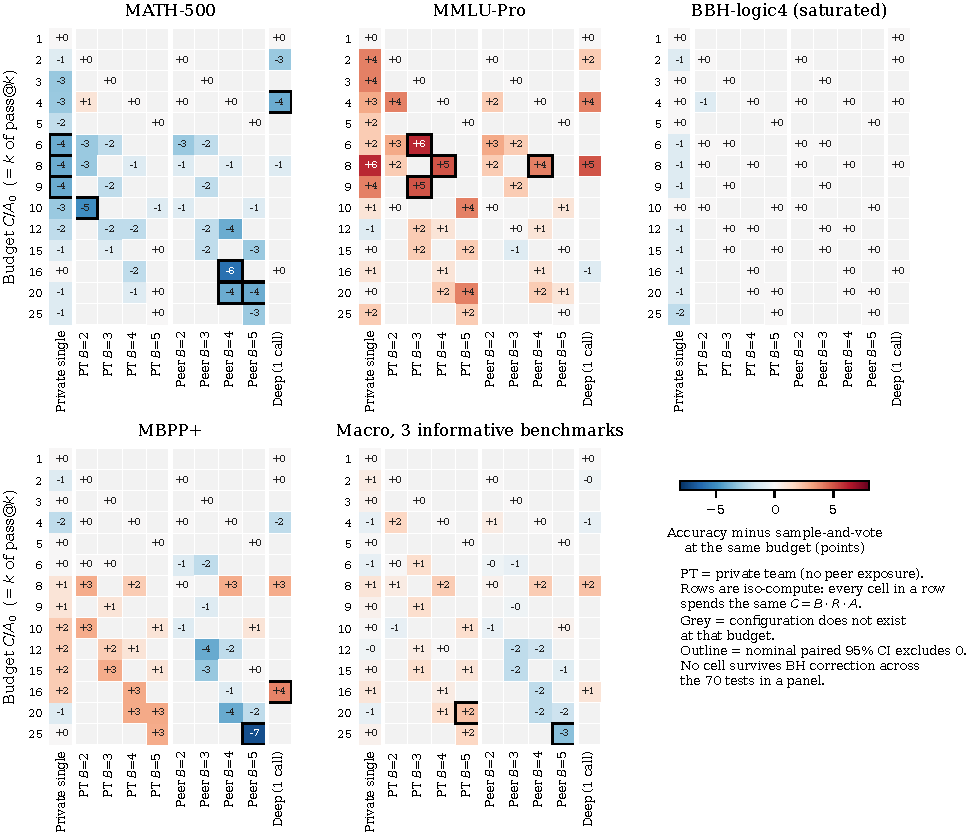
\includegraphics[width=0.99\textwidth]{figures/f3a_amplification_delta.pdf}
\caption{Amplification relative to sampling. Rows are iso-compute budgets; every cell in a row
spends the same $C$. Values are delivered accuracy minus sample-and-vote at that budget, in
accuracy points. Outlines mark nominal paired intervals excluding zero; \emph{no} cell survives
Benjamini-Hochberg control across the 70 tests in a panel. PT is a private team, that is, a team
without peer exposure.}
\label{fig:matrix}
\end{figure}

The matrix is mostly pale, and that is the result. Across 70 comparisons per benchmark, zero
survive multiplicity correction; the smallest $p$-value on the macro is 0.017, far above the
Benjamini-Hochberg threshold. Only 2 macro cells and 8 MATH-500 cells clear even an uncorrected
interval. A practitioner choosing among these allocations at fixed cost is, on this evidence,
choosing among options that cannot be reliably distinguished.

The signs are nonetheless consistent and worth reading. Private teams sit on the positive side on
MMLU-Pro (up to $+6$ points) and MBPP+ (up to $+3$), and on the negative side on MATH-500. Peer
configurations sit on the negative side almost everywhere and grow more negative toward the bottom
of the matrix, that is, at larger budgets with more rounds. The \texttt{deep} column is positive on
MBPP+ ($+3$ to $+4$) and negative on MATH-500.

Figure~\ref{fig:capture} normalises the same comparison against the headroom available at each
budget.

\begin{figure}[htbp]
\centering
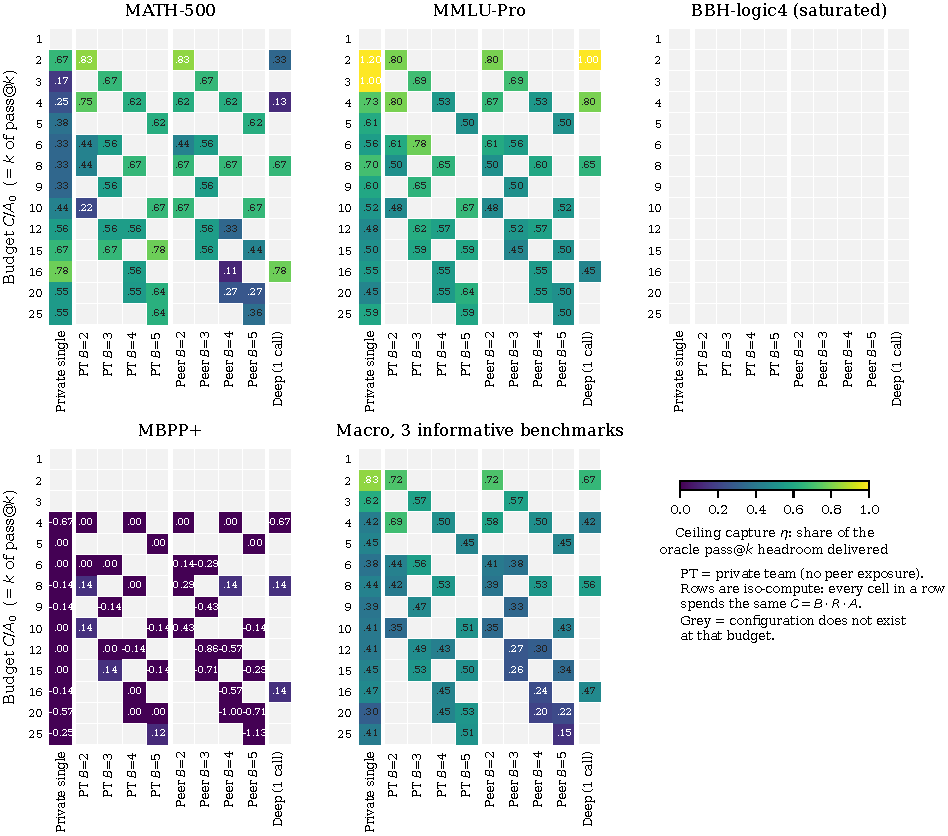
\includegraphics[width=0.99\textwidth]{figures/f3b_ceiling_capture.pdf}
\caption{Ceiling capture $\eta$: the share of the headroom a budget makes available that the
configuration actually delivers. BBH is masked because its denominator is zero.}
\label{fig:capture}
\end{figure}

Capture falls as budget rises. On the macro the median $\eta$ is 0.67 at the smallest budgets and
0.39 by $C/A_0 \geq 16$; on MMLU-Pro it falls from 0.80 to 0.50. On MBPP+ the median capture at
large budgets is $-0.25$, meaning the typical configuration there ends up below a single sample
even as coverage improves. The one cell above 1.0, a single agent revising once on MMLU-Pro, is
genuine: revision produced correct answers that neither independent sample contained.

\subsection{Width against depth}

Figure~\ref{fig:wd} isolates the shape question by fixing the budget and varying only how it is
split.

\begin{figure}[htbp]
\centering
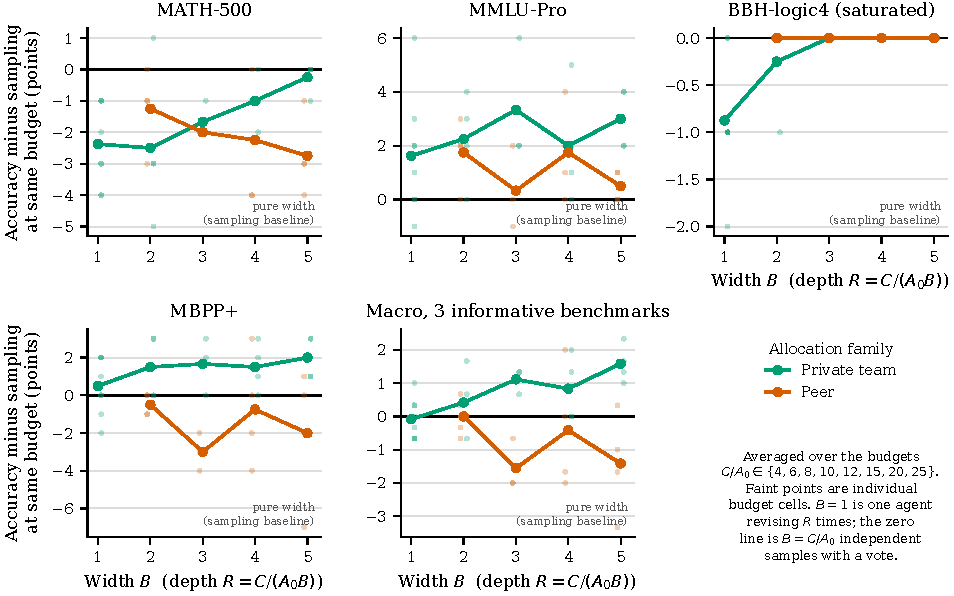
\includegraphics[width=\textwidth]{figures/f4_width_vs_depth.pdf}
\caption{Allocation shape at fixed compute, averaged over budgets $C/A_0 \in \{4,6,8,10,12,15,20,25\}$.
$B{=}1$ is one agent revising $R$ times. The zero line is the same budget spent on $B = C/A_0$
independent samples.}
\label{fig:wd}
\end{figure}

For private teams, wider is mildly better than deeper: on the macro the mean amplification rises
from about $0$ at $B{=}1$ to $+1.6$ points at $B{=}5$, and the same upward slope appears on
MATH-500, MMLU-Pro and MBPP+. Pure depth, one agent revising many times, is the weakest private
allocation on every informative benchmark. For peer configurations the slope is absent or reversed
and the whole curve sits below zero on the macro and on MBPP+.

Two readings follow. Spreading a budget across a few agents is slightly better than spending it on
one agent thinking for longer in sequence, but the advantage is within noise. And the gap between
the private and peer curves, which is the pure effect of letting agents see each other, is larger
and more consistent than the width-depth effect it is plotted against.

\subsection{Generation is not the bottleneck}

Figure~\ref{fig:gap} makes the central claim directly.

\begin{figure}[htbp]
\centering
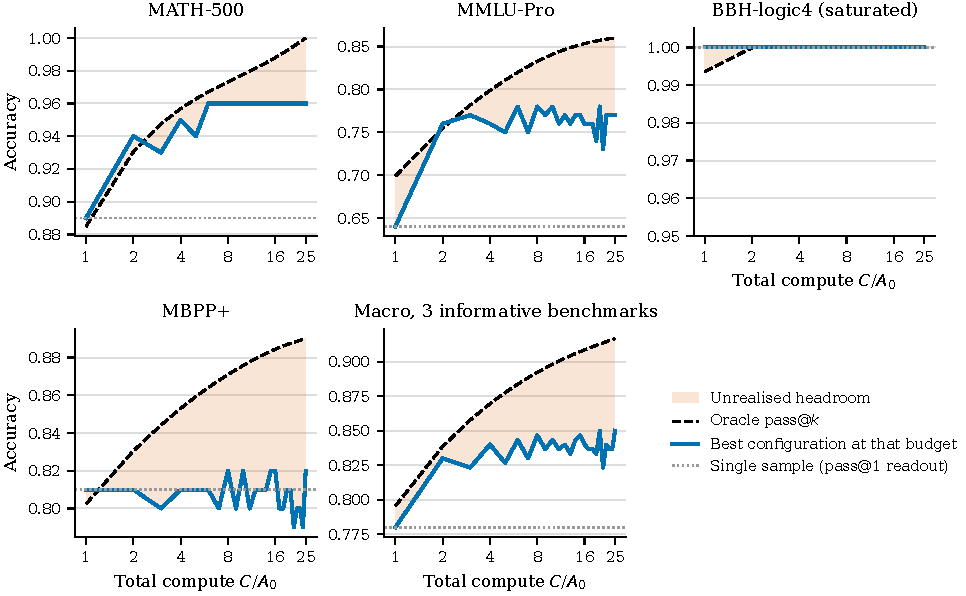
\includegraphics[width=\textwidth]{figures/f5_selection_gap.pdf}
\caption{The selection gap. The shaded band is headroom that compute made available and no
evaluated configuration collected. The blue line is the maximum over all configurations at that
budget, so it is an optimistic envelope and still falls short.}
\label{fig:gap}
\end{figure}

At the largest budget the best configuration on the macro reaches 0.850 against an oracle of 0.917,
leaving 6.7 points unrealised. Per benchmark the unrealised headroom is 4.0 points on MATH-500, 9.0
on MMLU-Pro and 7.0 on MBPP+. The band widens monotonically: at $C = 2A_0$ it is near zero, and
every additional unit of compute after that adds more to the ceiling than to what any policy
delivers.

The blue line is deliberately generous. It takes the maximum over up to seven configurations at
each budget, so it is biased upward by selection on this very sample, and the gap is still large.

\subsection{The cost of letting agents talk}

The one prespecified contrast that resolves is the comparison between teams that see each other and
teams that do not, at matched size and matched rounds.

\begin{tabular}{llrrrr}
\toprule
Contrast & Level & $n$ & Estimate & 95\% CI & Holm $p$ \\
\midrule
Peer $-$ private team, $B$=4, $r$=4 & Macro (4) & 400 & -0.0250 & [-0.046, -0.008] & 0.027 \\
\quad & MATH-500 & 100 & -0.0300 & [-0.064, -0.003] & n/a \\
\quad & MMLU-Pro & 100 & +0.0000 & [+0.000, +0.000] & n/a \\
\quad & BBH-logic4 & 100 & +0.0000 & [+0.000, +0.000] & n/a \\
\quad & MBPP+ & 100 & -0.0700 & [-0.144, -0.010] & n/a \\
\midrule
CP $-$ private-team gain, $h$=3 & Macro (4) & 192 & -0.0052 & [-0.025, +0.009] & 0.567 \\
\quad & MATH-500 & 48 & -0.0208 & [-0.021, +0.004] & n/a \\
\quad & MMLU-Pro & 48 & +0.0000 & [+0.000, +0.000] & n/a \\
\quad & BBH-logic4 & 48 & +0.0000 & [+0.000, +0.000] & n/a \\
\quad & MBPP+ & 48 & +0.0000 & [-0.053, +0.053] & n/a \\
\bottomrule
\end{tabular}


Peer exposure at four agents and four rounds costs 2.50 accuracy points on the four-benchmark macro,
with a 95\% interval of $[-0.046, -0.008]$ and a Holm-corrected $p$ of 0.027. The effect is carried
by MBPP+ ($-7.0$ points) and MATH-500 ($-3.0$); it is exactly zero on MMLU-Pro and on saturated BBH.
The second prespecified contrast, the communicate-then-private decomposition at $h{=}3$, is null at
$-0.005$ with $p = 0.567$.

Figure~\ref{fig:comm} shows that this is not a single unlucky cell but a trend.

\begin{figure}[htbp]
\centering
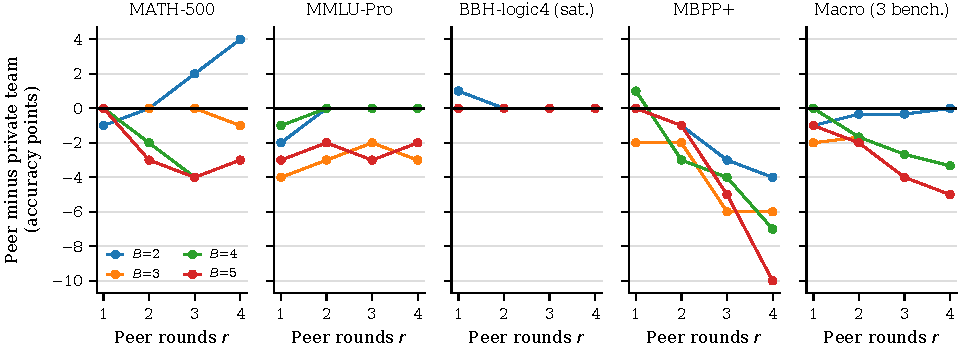
\includegraphics[width=\textwidth]{figures/f6_communication_cost.pdf}
\caption{Peer minus private team at matched team size and matched rounds. The only difference
between the two arms is whether agents see each other's drafts.}
\label{fig:comm}
\end{figure}

The penalty deepens with rounds on every informative benchmark and with team size on MBPP+. At the
largest configuration, five agents and four peer rounds, the cost is 5.0 points on the macro
($[-0.077, -0.023]$) and 10.0 points on MBPP+ ($[-0.17, -0.04]$).

Figure~\ref{fig:dyn} shows the mechanism. Revision rounds move a substantial number of answers in
both directions, and the net is close to zero.

\begin{figure}[htbp]
\centering
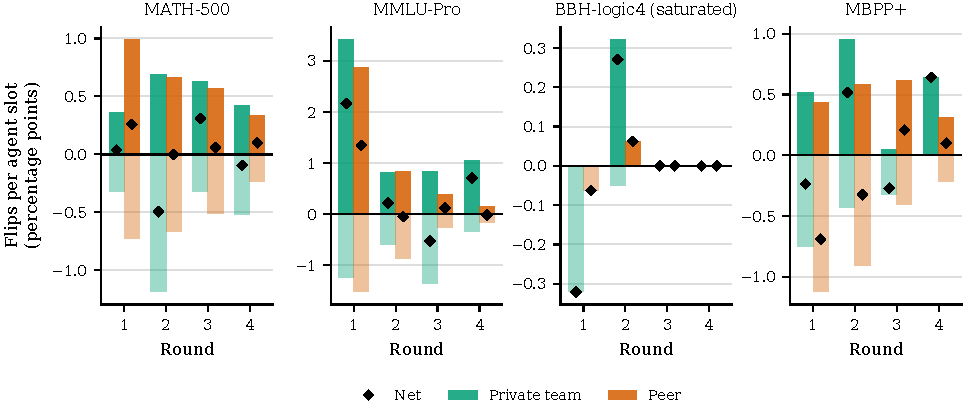
\includegraphics[width=\textwidth]{figures/f7_round_dynamics.pdf}
\caption{Churn per revision round. Solid bars are wrong-to-correct flips, faded bars are
correct-to-wrong, and the diamond is the net. Rates are per agent slot, in percentage points.}
\label{fig:dyn}
\end{figure}

On MMLU-Pro the first round has a clearly positive net and later rounds do not, which is why one
revision round is the best MMLU-Pro configuration in the whole design. On MATH-500 and MBPP+ the
net is negative for several rounds. Peer exposure raises the correct-to-wrong rate more than it
raises the wrong-to-correct rate, which is exactly the shape of a consensus process that propagates
confident errors.

\subsection{Depth inside one call}

The \texttt{deep} arm spends the whole budget on a single call with a larger reasoning allowance,
so it pays no repeated prompt cost and has no opportunity to select.

\begin{figure}[htbp]
\centering
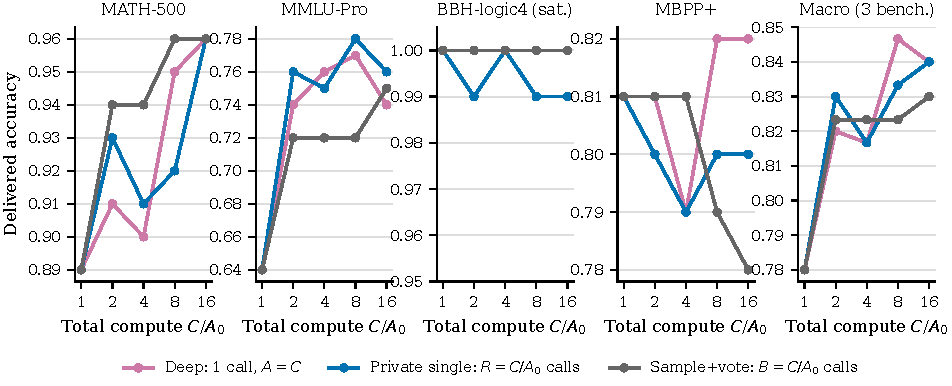
\includegraphics[width=\textwidth]{figures/f8_depth_one_call.pdf}
\caption{The same budget as one long call, as sequential revisions, or as parallel samples.}
\label{fig:deep}
\end{figure}

One deeper call is competitive with everything else and is the single best configuration on MBPP+
(0.820 at $C = 8A_0$, against 0.790 for eight samples). On the macro it reaches 0.847, within 0.3
points of the best configuration in the entire design, using one generation rather than twenty.
On MATH-500 it trails sampling slightly. Since it requires no orchestration, no repeated context and
no selector, it is the most practical of the allocations tested.

\subsection{What this costs in dollars}

\begin{figure}[htbp]
\centering
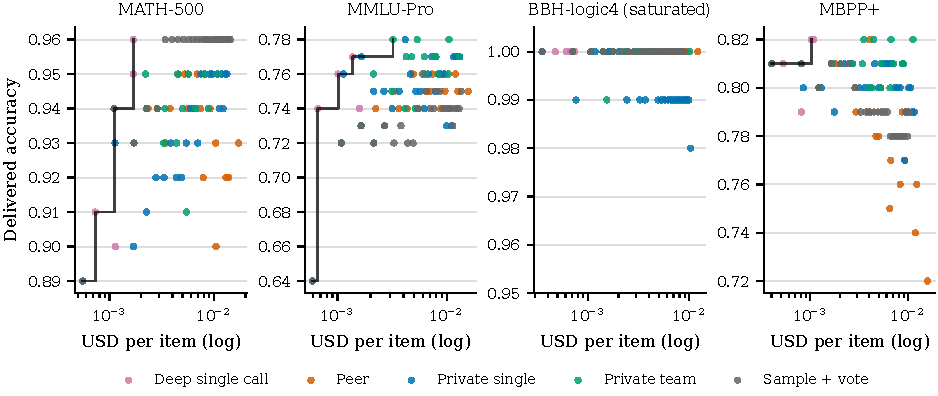
\includegraphics[width=\textwidth]{figures/f9_dollar_frontier.pdf}
\caption{Delivered accuracy against realised spend per item. The step line is the descriptive
Pareto front over evaluated configurations.}
\label{fig:dollar}
\end{figure}

The frontier saturates almost immediately. One sample costs \$0.000475 per item and one deeper call
at $8A_0$ costs \$0.001207; five agents over four peer rounds cost \$0.015196, which is 32 times the
single sample, and deliver less. Everything beyond the deeper single call at \$0.001207 per item is, on this
evidence, spent without return.

\subsection{Robustness}

\begin{figure}[htbp]
\centering
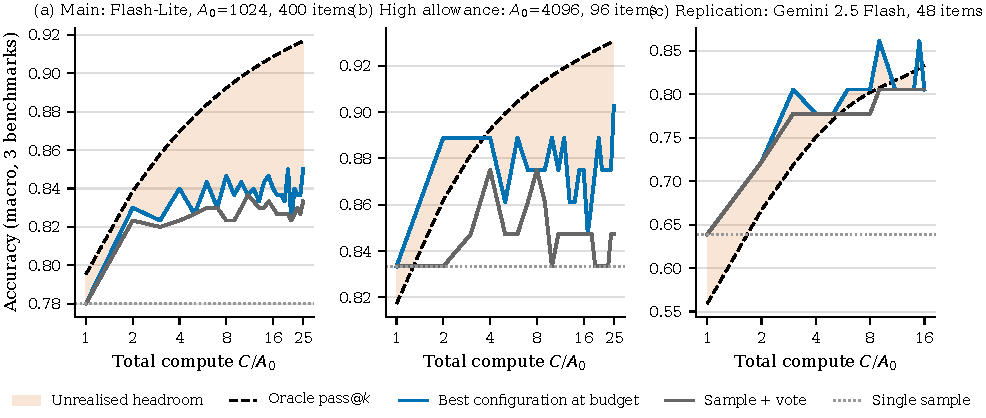
\includegraphics[width=\textwidth]{figures/f10_robustness.pdf}
\caption{The same comparison at four times the reasoning allowance and on a stronger model, on
shared items only. The 96-item and 48-item panels have unstable intervals.}
\label{fig:robust}
\end{figure}

Raising the allowance to $A_0 = 4096$ lifts the whole picture, with pass@1 at 0.833 and the best
configuration reaching 0.903, but the qualitative shape survives: the ceiling is 0.931 and 2.8
points remain unrealised. The Gemini 2.5 Flash replication behaves the same way, with a best
configuration of 0.806 against a ceiling of 0.833 at $k=16$. Both panels are small, 96 and 48 items,
so these are consistency checks rather than independent confirmations. The direction of the peer
penalty is preserved on both.

\subsection{Anatomy of the gap}

Every configuration satisfies, per item, \emph{delivered} = \emph{pool coverage} $-$
\emph{selection loss}, where coverage is 1 when the configuration's own candidate pool contained a
correct answer. Comparing that coverage with independent sampling at the same budget splits the gap
in two: a generation-side part, where the pool never held the answer, and a selection-side part,
where it did and the selector missed it.

\begin{tabular}{lrrrrr}
\toprule
Allocation & Pool coverage & Delivered & Coverage deficit & Selection loss & Archive \\
\midrule
\texttt{private\_team/5/4} & 0.903 & 0.850 & 0.013 & 0.053 & 0.850 \\
\texttt{private\_single/25} & 0.837 & 0.837 & 0.080 & 0.000 & 0.840 \\
\texttt{sample/25} & 0.917 & 0.833 & 0.000 & 0.083 & 0.833 \\
\texttt{peer/5/4} & 0.807 & 0.800 & 0.110 & 0.007 & 0.837 \\
\midrule
\emph{Sampling ceiling} & 0.917 & & & & \\
\bottomrule
\end{tabular}


The split is stark. Independent sampling has \emph{zero} coverage deficit by construction and its
entire 8.3-point gap is selection loss. One agent revising 25 times has the opposite profile:
essentially no selection loss, because its delivered pool is a single final answer, and an 8.0-point
coverage deficit. Peer teams are worst on coverage, at 11.0 points, because mutual exposure
collapses the pool onto a shared answer. No allocation in the study is generation-limited in the
sense that matters: at every budget, some allocation holds the correct answer.

\begin{figure}[htbp]
\centering
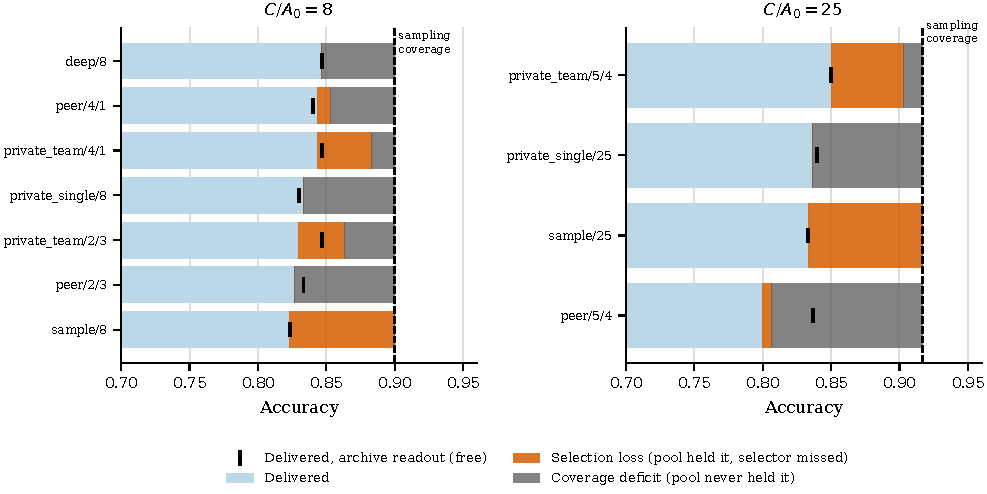
\includegraphics[width=\textwidth]{figures/f12_gap_split.pdf}
\caption{Each allocation's budget-matched gap, split into the two losses. Bars sum to the coverage
that independent sampling achieves at the same budget. Tick marks show the archive readout, which
votes over every round's output instead of only the last and costs nothing extra.}
\label{fig:split}
\end{figure}

Figure~\ref{fig:anatomy} explains why coverage is nearly worthless on its own. Given that a correct
answer is in the pool, the probability of delivering it is 0.305 on MATH-500, 0.20 on MMLU-Pro and
0.06 on MBPP+ when correct answers make up under a fifth of the pool, and rises to essentially 1 on
the text benchmarks once they pass half. A vote does not need the correct answer to be present, it
needs it to be modal.

\begin{figure}[htbp]
\centering
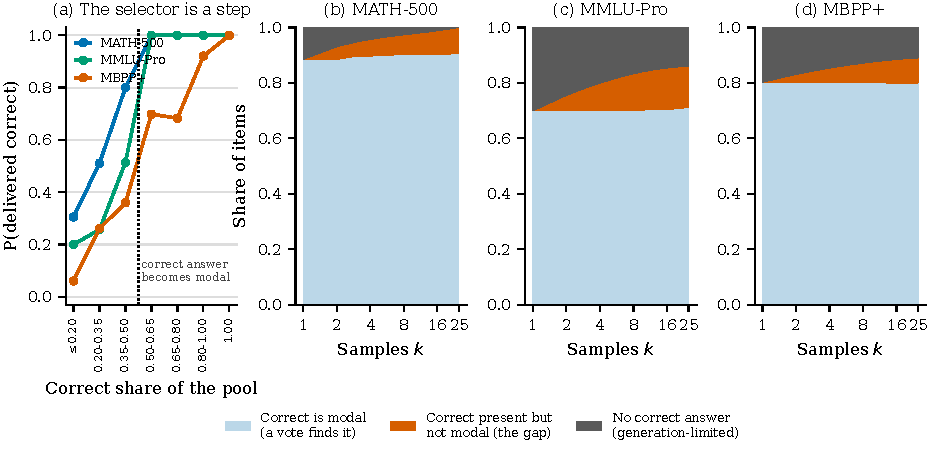
\includegraphics[width=\textwidth]{figures/f11_gap_anatomy.pdf}
\caption{(a) Probability of delivering a correct answer given that one is in the pool, against the
correct share of that pool. (b to d) Where the item mass sits for a $k$-sample prefix, computed
exactly from the bank by the hypergeometric prefix distribution, with ties broken as half.}
\label{fig:anatomy}
\end{figure}

That is what the stacked panels show. On MMLU-Pro, going from one sample to twenty-five reduces the
share of items with no correct answer anywhere from 0.301 to 0.140. Almost none of that 16.1 points
becomes deliverable: the majority share rises only from 0.699 to 0.710, and 15.0 points land in the
middle band where a correct answer exists and loses the vote. Extra draws convert impossible items
into unusable ones. The middle band is the oracle gap, exactly.

The archive readout is the one free lever. Voting over every round's output rather than the last
restores \texttt{private\_team/5/4} coverage to 0.917, precisely the 25-sample ceiling, at no extra
tokens. As a delivered gain it is worth $+0.037$ on \texttt{peer/5/4} (95\% CI $[0.017, 0.060]$) and
$+0.033$ on \texttt{peer/4/4}, but only $0.000$ on \texttt{private\_team/5/4}. It repairs what peer
exposure discards; it does not lift the frontier.

\subsection{What a verifier would buy}

If selection is the constraint, the natural question is how good a selector would have to be.
Figure~\ref{fig:verifier} answers it on the real pool compositions by scoring correct candidates
$\mathcal{N}(\mu, 1)$ and incorrect ones $\mathcal{N}(0,1)$ and taking the argmax, which makes the
verifier's pairwise AUC $\Phi(\mu/\sqrt{2})$.

\begin{figure}[htbp]
\centering
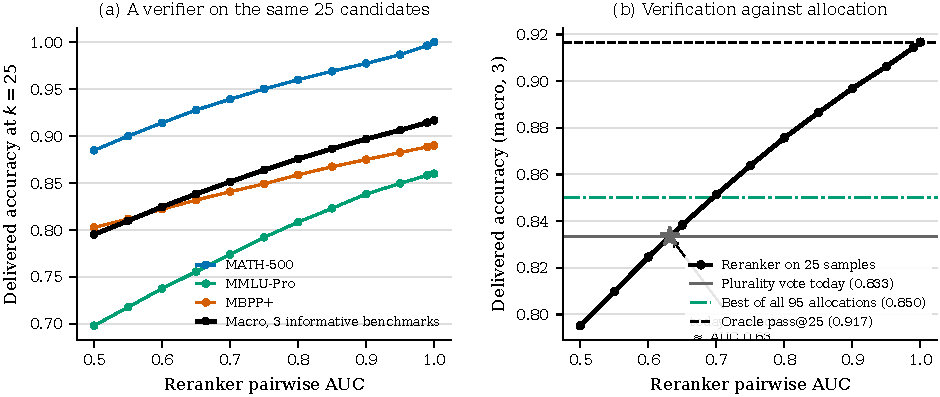
\includegraphics[width=\textwidth]{figures/f13_verifier_sweep.pdf}
\caption{Delivered accuracy at $k=25$ from a reranker of given pairwise AUC, applied to candidates
the run already generated. This bounds what discriminative power is worth; it is not evidence that
such a verifier exists for these tasks.}
\label{fig:verifier}
\end{figure}

Today's plurality vote delivers 0.833 on the macro, which is what a reranker of AUC 0.63 would
achieve. A reranker at AUC 0.70 delivers 0.851, already above the best of all 95 allocations
(0.850). At AUC 0.80 it delivers 0.876, which is 2.6 points beyond anything the allocation design
reached, and at AUC 0.90 it delivers 0.897 against an oracle of 0.917.

The comparison is the point. The entire design, 95 configurations and 67{,}514 generations spanning
every combination of agents, rounds and reasoning allowance, moves delivered accuracy over a range
of about 7 points. A mediocre verifier applied to twenty-five samples already paid for moves it
further.

\subsection{The one generation-side lever, and one selector that backfires}

\begin{figure}[htbp]
\centering
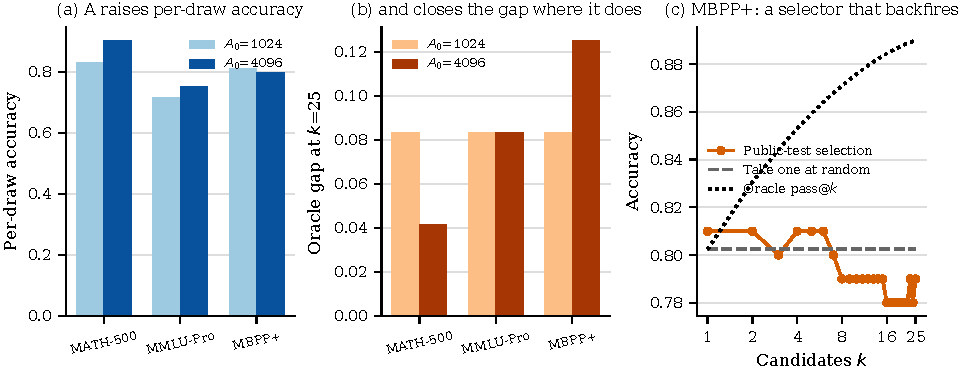
\includegraphics[width=\textwidth]{figures/f14_allowance_and_selector.pdf}
\caption{(a, b) The reasoning allowance on the 96 shared items. (c) MBPP+ public-test selection
against simply taking one candidate at random.}
\label{fig:allowance}
\end{figure}

Because the gap is governed by per-draw accuracy rather than draw count, the one axis that should
help is $A$. On the 96 shared items, raising the allowance from 1024 to 4096 lifts MATH-500 per-draw
accuracy from 0.830 to 0.902 and halves the gap from 0.083 to 0.042. On MMLU-Pro per-draw accuracy
rises from 0.717 to 0.753 and the gap is unchanged at 0.083. On MBPP+ per-draw accuracy falls
slightly and the gap widens from 0.083 to 0.125. $A$ helps exactly where longer reasoning raises
per-draw accuracy, and not otherwise.

Among allocations, the only lever that moves the relevant quantity is concentration. At $C = 25A_0$
private teams raise the correct share of the pool from 0.795 under sampling to 0.843, which is why
they deliver 0.850 against 0.833. Peer exposure lowers it to 0.797. Private teams help not because
they explore more but because they consolidate, which is what a vote can use.

Finally, one defect worth fixing on its own. MBPP+ selects by prompt-visible tests, and from $k=8$
onward that selector performs \emph{below} a random draw: 0.790 against 0.802 at $k=25$, having
started at 0.810 for a single candidate. Enlarging a code candidate pool and filtering on visible
assertions finds programs that satisfy the visible evidence and fail the hidden suite. On this
benchmark the run would have done better selecting at random, and better still doing nothing.

\subsection{Does the allocation change how well a pool reads out?}

Delivering a correct answer requires the pool to hold one, so for every configuration
\emph{delivered} $=$ \emph{coverage} $\times S$ exactly, where $S$ is selection success, the chance
of delivering given the pool held a correct answer. That identity turns the allocation question
into a question about which of the two factors an axis buys.

\begin{figure}[htbp]
\centering
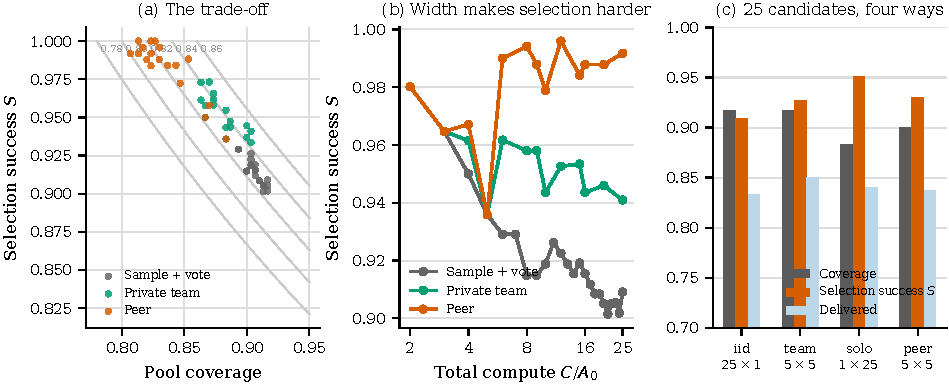
\includegraphics[width=\textwidth]{figures/f15_coverage_selectability.pdf}
\caption{(a) Every configuration at $C/A_0 \geq 4$ in the coverage-selectability plane; grey lines
are iso-delivered contours, since the product of the axes is delivered accuracy. Private single is
absent because its current-view pool is one candidate, so it has no selection to measure.
(b) Selection success against budget. (c) Four ways to produce 25 candidates.}
\label{fig:tradeoff}
\end{figure}

The answer is that allocation changes selection success a great deal, and in the direction opposite
to its effect on coverage. Scaling horizontally drives $S$ down: independent sampling falls from
0.965 at the smallest budgets to 0.905 at the largest, because each extra candidate is another way
for the vote to fragment. Scaling vertically with peer exposure drives $S$ up, from 0.970 to 0.989,
because the agents converge on one answer and the vote becomes trivial. Private teams sit between,
at 0.967 falling to 0.944.

Neither extreme wins, because each pays for its factor with the other. Peer configurations have the
best selection success in the entire study and the worst coverage; independent sampling has the
best coverage and the worst selection success. Panel (a) shows the consequence: the configurations
lie along an anti-diagonal band and therefore mostly on the same iso-delivered contour. This is the
mechanism behind the report's first finding. Allocation shape is close to irrelevant not because
the axes do nothing, but because what they give on one factor they take back on the other.

The controlled comparison is panel (c), where pool size is held at 25 and only the way those 25
candidates were produced varies. Twenty-five independent samples and a five-agent, five-round team
read over its archive have \emph{identical} coverage, 0.917. The team's pool is more concentrated,
0.829 against 0.795, and its selection success is higher, 0.927 against 0.909, so it delivers 0.850
against 0.833. The difference is $+0.017$ with a 95\% interval of $[-0.003, 0.037]$, so the
mechanism is measured cleanly while the delivered advantage is not separable from noise at 400
items. One agent revising 25 times has the highest selection success of all, 0.951, and loses on
coverage, at 0.883.

The practical reading is that a mix is the only allocation that can hold both factors at once:
parallel agents give coverage, revision gives concentration, and reading out over the archive
rather than the final round keeps both. That is a reason to prefer it, but this study does not
have the power to prove it pays.

\subsection{Repairing the selector}

If selection is the constraint, the structure of the answer space decides which repair is even
available. Figure~\ref{fig:repair} shows that this structure differs enormously across benchmarks.

\begin{figure}[htbp]
\centering
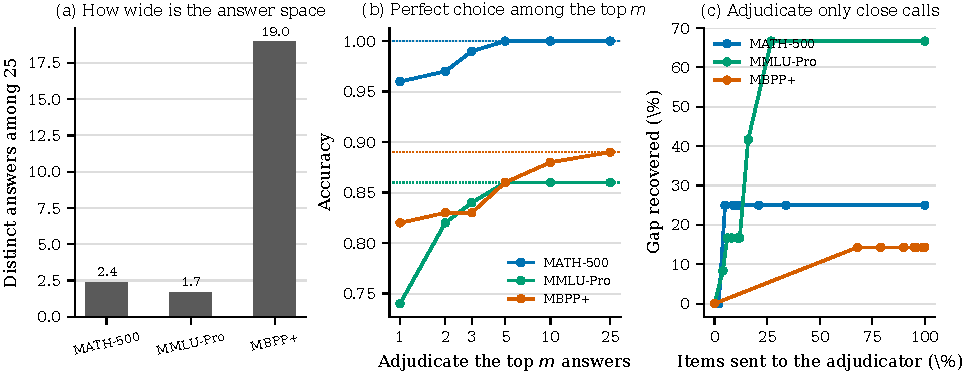
\includegraphics[width=\textwidth]{figures/f16_selection_repair.pdf}
\caption{(a) Distinct answers among 25 samples. (b) Accuracy from a perfect choice restricted to the
$m$ most-voted distinct answers; dotted lines are each benchmark's oracle. (c) Gap recovered against
the share of items sent to an adjudicator, gating on the plurality margin.}
\label{fig:repair}
\end{figure}

Twenty-five MMLU-Pro samples produce only 1.7 distinct answers, with the top one taking 0.891 of
the vote. MATH-500 produces 2.4. MBPP+ produces 19.0, with the top program taking 0.170, because
programs are nearly all textually unique. These are three different selection problems wearing the
same name.

Where the answer space is narrow, the repair is cheap. On MMLU-Pro a perfect choice between just the
\emph{top two} voted answers lifts accuracy from 0.740 to 0.820, which is $+0.080$ with a 95\%
interval of $[0.030, 0.140]$ and recovers two thirds of the 0.120 gap. By the top five it reaches
0.860, the full oracle. On the twelve items where a correct answer exists and the vote misses it,
the correct answer is ranked second in two thirds of cases and ranked 2.58 on average. So the
verifier this benchmark needs is not a reranker over 25 candidates; it is one binary comparison per
item.

Where the answer space is wide, adjudication does almost nothing. On MBPP+ the correct program sits
at rank 7.43 among the failing items, top-two adjudication is worth $+0.010$ $[0.000, 0.030]$, and
recovering the gap requires ranking essentially the whole pool. Code needs a verifier that scores
each candidate on its own, which in practice means better tests rather than better voting. That is
consistent with the public-test selector failing here: it is the only benchmark whose selector
already tries to score candidates individually, and it does so on evidence the candidates were
optimised against.

Gating helps less than it should. Sending only the closest 16\% of MMLU-Pro items to an adjudicator
recovers 0.417 of the gap, and recovering the full 0.667 requires sending all of them. The reason is
visible in panel (a): the mean plurality margin on MMLU-Pro is 0.813, so most failures are not close
calls. They are items where the model is confidently and consistently wrong, and an adjudicator has
to be willing to overrule a large majority. That is a harder verifier to build than a tie-breaker,
and it is the central difficulty this study surfaces.

\subsection{A design check}

On all 400 items, a team of $n$ agents run for zero revision rounds delivers exactly the same answer
as $n$ independent samples, under both the private and the peer arms. This is true by construction,
since with no rounds there is nothing to revise and nothing to see, and its exact agreement
(400 of 400 items for every $n$) confirms that the iso-compute re-keying used throughout this report
lines up with the sealed selection records.

\section{Interpretation}

\textbf{At fixed compute, the shape of the allocation is close to irrelevant.} This is the least
exciting reading of the data and the best supported one. Seventy paired comparisons per benchmark
produce no effect that survives correction, and the spread across all allocations at the largest
budget is about 5 accuracy points on the macro, comparable to the width of a single confidence
interval. Claims that multi-agent structure beats single-agent inference should be checked against a
compute-matched sampling baseline, because on this model and these benchmarks that baseline is
already most of the way to the best result anyone achieves.

\textbf{Test-time compute keeps working; test-time \emph{selection} does not.} Oracle pass@$k$
rises steadily and without any sign of saturating below 0.92 on the macro, which means additional
compute is still producing correct answers. What fails is the readout. Plurality voting stops
improving after roughly two samples, and on MBPP+ the public-test selector gets actively worse as
the pool grows, because more candidates means more candidates that satisfy the visible evidence and
fail the hidden suite. The gap between what was generated and what was delivered is the largest
single quantity in this study, and it grows with every dollar spent.

\textbf{Communication between agents is a cost, not a benefit, in this regime.} The prespecified
contrast is negative and significant, the effect deepens monotonically with rounds, and the round
dynamics show why: peer exposure increases the rate at which correct answers become wrong more than
it increases the reverse. A small model shown its peers' drafts converges, and convergence on a
wrong answer is indistinguishable at readout time from convergence on a right one. The private team,
which gets the same number of agents and rounds with no mutual visibility, dominates it everywhere.
This should be read as a statement about small models with a plurality readout, not about
multi-agent debate in general, but it does mean the burden of proof runs the other way.

\textbf{Width beats depth slightly, and one deeper call beats both on cost.} Among private
allocations, spreading a budget over three to five agents edges out spending it on one agent
revising many times, though the margin is inside the noise. More striking is that a single call with
the whole budget as reasoning allowance matches the best orchestrated configuration on the macro to
within 0.3 points and wins outright on MBPP+, while requiring no orchestration, no repeated context
and no selector. If a practitioner has to pick one thing to do with extra tokens on this model, the
evidence points at that.

\textbf{A prescription, in order of what it is worth.} The levers can be ranked on this data, at
$C = 25A_0$ on the three-benchmark macro.

\emph{First, verification.} Moving the selector from its current effective AUC of 0.63 to 0.80 is
worth 4.3 points, from 0.833 to 0.876, on candidates already generated. Even AUC 0.70 beats every
allocation in the study. Nothing else on this list comes close, and it is the only lever that scales
with the compute already being spent, because a better selector makes every additional sample worth
something.

\emph{Second, per-draw reasoning.} Raising $A$ is the only generation-side axis that touches the
binding quantity, and it works where longer reasoning raises per-draw accuracy: it halved the
MATH-500 gap, did nothing on MMLU-Pro and hurt on MBPP+. Verify per benchmark before spending on it.

\emph{Third, fix broken selectors.} MBPP+ public-test selection is below random from $k=8$. This is
not a research problem, it is a defect, and repairing it is worth 1.2 points immediately and unlocks
the 10-point coverage headroom that sits behind it.

\emph{Third-and-a-half, adjudicate the top two where the answer space is narrow.} On MMLU-Pro one
binary comparison per item is worth $+0.080$ $[0.030, 0.140]$, two thirds of the gap, and needs a
single extra call rather than a full reranking pass. This does not transfer to code, where the
correct program ranks 7.43 among failures and no shortlist is short enough.

\emph{Fourth, consolidate rather than communicate.} If the readout is a vote, prefer allocations that
raise the correct share of the pool. Private teams do this and are worth 1.7 points over sampling;
peer exposure does the opposite. Read out over the archive rather than the last round, which is free
and recovers 3.7 points of the damage peer exposure causes.

\emph{Last, and close to worthless, more draws.} At fixed $A$ with a vote as the readout, additional
agents or rounds move delivered accuracy by about nothing. They raise the ceiling and leave the
floor where it is.

The one-line version: this model does not need to think more times, it needs someone to tell it
which of its answers was right.


\appendix

\section{A validation experiment for the prescription}

The prescription rests on a simulation: a reranker of given pairwise AUC, applied to the pool
compositions this run actually produced. It bounds what discriminative power is worth. It does not
show that a verifier with that power is available for these tasks. The following design tests that,
and it is cheap because the candidates already exist.

\textbf{Hypothesis.} A judge model scoring stored candidates delivers higher accuracy at $k=25$ than
the plurality vote, by at least the 4.3 macro points the simulation predicts for AUC 0.80.

\textbf{Design.} No generation. The 25-sample bank for each of the 400 main-panel items is already
stored, graded and sealed, so the run scores existing candidates and re-reads the outcome. Arms:

\begin{enumerate}
\item \emph{Pointwise judge}, Flash-Lite. One call per candidate scoring correctness on a fixed
rubric without the reference answer. 10{,}000 calls.
\item \emph{Pointwise judge}, Flash, as a capability check on the same items.
\item \emph{Top-two adjudication}, one pairwise call per item between the two most-voted answers.
On the analysis above this is the highest-value arm on MMLU-Pro and the cheapest to run, at 400
calls rather than 10{,}000. It also tests the hard part directly, since the adjudicator must be
willing to overrule a majority whose mean margin is 0.813.
\item \emph{MBPP+ selector repair}, at zero API cost: re-select among stored candidates that pass the
public assertion, breaking ties by judge score rather than by order.
\end{enumerate}

\textbf{Primary outcome.} Delivered accuracy at $k=25$, macro over the three informative benchmarks,
paired per item against the sealed plurality readout. \textbf{Secondary.} The judge's realised
pairwise AUC, which places it on Figure~\ref{fig:verifier} and tests the simulation itself rather
than only its conclusion.

\textbf{Power.} The median standard error of a paired macro contrast on this panel is 0.0119 at 400
items, so the minimum detectable effect at 80\% power is 0.0333. The predicted effect of 0.043
clears it; a 192-item panel, with a detectable effect of 0.0481, would not. Use the full 400 items.

\textbf{Cost.} At roughly 1082 completion tokens per stored candidate, the pointwise arm is about
16.8M input and 1.28M output tokens: \$2.19 on Flash-Lite and \$8.25 on Flash. The pairwise arm adds
ten comparisons per item. The whole study is comfortably inside \$25, against \$47.64 already spent
of a \$135 ledger ceiling. The shared account balance should be checked before launching, since it
is not reserved for this study.

\textbf{Prespecify before running.} The rubric and its version hash, the scoring temperature, the
tie-break rule, the exclusion of the reference answer from the judge context, and the two primary
comparisons (pointwise judge against plurality, and pairwise against pointwise) with Holm
correction over exactly those two. The judge must never see the grader output; the existing
seal-before-join discipline applies unchanged.

\textbf{What would falsify the prescription.} If a competent judge lands at or below AUC 0.63, which is what plurality already achieves, the
selection headroom identified here is not reachable with an LLM judge on these tasks, and the
conclusion narrows from ``spend on verification'' to ``this particular verifier does not work'', with
the gap remaining open.

\end{document}
